%%%%%%%%%%%%%%%%%%%%%%%%%%%%%%%%%%%%%%%%%%%%%%%%%%%
%%% CONCLUSIONES Y TRABAJO FUTURO
%%%%%%%%%%%%%%%%%%%%%%%%%%%%%%%%%%%%%%%%%%%%%%%%%%%

\chapter{Conclusions and Future Work}
\fancyhead[RE]{\textsc{Chapter} \thechapter. Conclusions and Future Work}
\label{ch:ConclusionsAndFutureWork}
\section{Conclusions}
\label{sec:Conclusions}
\noindent To explain \emph{black box} models such as deep learning models it is a really complex task that, despite of the efforts of the researchers, is still a challenge far away from being completely solved. 
\paragraph{}
Among the last years researchers have developed some interesting approaches that are really helpful to understand the model behaviour and to know a bit more about why the model has given an output instead of another one. These approaches are based on some different techniques that help the user to understand what is going on inside the model when giving an output, and to make it easier for the user are often presented with visualization tools and techniques that make really simple to understand the explanations. 
\paragraph{LIME} After several experiments, it can be seen that \emph{LIME} is able to detect the most important words (or spans) the model focus on when making its prediction. But it's still not clear why the model makes a prediction, because \emph{LIME} explains the most important words for each class, but does not explain why the model choose a class over the other ones.
\paragraph{}
This way, \emph{LIME} can help to understand the words that are important for the prediction, an this can help to understand the best way to create questions or to give the model the correct options. But it have been also seen that to change this words or this options does not mean the model is going to change its prediction. For instance, in the experiments in which the most important word ``discipline'' was replaced with a synonym ``orderliness'', the model predicted the good label meanwhile with the word ``discipline'' that appeared in the original text the model did not, and in the experiment in which the options given to the model were perturbed trying to preserve all the important words in the original question (like ``supposed'') the model also failed in its prediction.
\paragraph{}
So it is not clear which one is the correct way to make a question, or why the model has chosen a class instead of another one.
Besides this, when the model fails, \emph{LIME} does not really help to know why the model has failed, because the explanations of each of the classes will give us the important words for that class, but will not tell why a class is chosen beyond the others. 
\begin{figure}[!h]
	\centering
	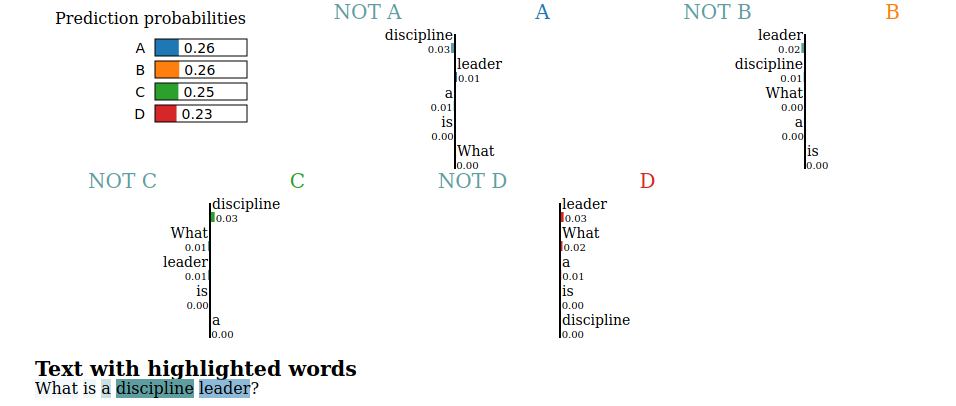
\includegraphics[scale=0.35]{images/conclussionLime}
	\caption{Explanation of all options given by \emph{LIME}}
	\label{fig:conclussionLime}
\end{figure}
\paragraph{BertVIZ} \emph{BertViz} is a tool to explote and visualize \emph{attention} weights in every \emph{transformer-based} model. It allows the user to visualize \emph{attention} weights in an easy and user-friendly way, making possible to see and detect bias and patterns in the \emph{attention} mechanism as well as to detect useless heads to be able to prune them and save space and time without loosing performance.
\paragraph{}
But, \emph{BertViz} is just that, a visualization tool. It does not provide or perform any additional operation over the model and, therefore, it does not help more than other visualization tools to understand what is going on inside the model. Although, as said before, it helps to visualize \emph{attention} weights to, for instance, detect patterns or see how words relate with others, this is not helpful when trying to understang the model behaviour and to know why the model has given an output and why not another one. But \emph{BertViz} is not guilty for this, because as some research articles\cite{} has pointed out recently, to visualize the \emph{attention} weights does not really provide an explanation of the local prediction, because the \emph{attention} mechanism is just used to generate contextual embeddings of the input. Instead of that it would be more useful to explain the final layers of the model, that are the ones that are really solving the task, but this is very difficult, as they have as input the embeddings generated by the full model, making it really difficult to explain the layers behaviour and to understand the explanations.
\paragraph{}
Therefore, other techniques such as \emph{LIME} that create a surrogate explainable model are more useful than to visualize the \emph{attention} weights in order to explain the model behaviour.
\section{FutureWork}
\label{sec:FutureWork} 